\section{El mètode principiants "Old Pochmann"}

El métode principiants o Old Pochmann és un mètode pel qual intercanvies les peces que vols una a una, és a dir, que mires la peça que primer has memoritzat i la canvies per la peça que està al seu lloc i així ja tens una peça que està al seu lloc i una altra que has de col·locar, i així succesivament.
Aquesta peça sobre la que sempre estàs treballant es diu "Buffer".El mètode és el mateix concepte tant per arestes com cantonades però el dividirem en dos perquè l'explicació sigui més fàcil.

\subsection{Arestes}

En les arestes el buffer serà la peça BM, (l'aresta blanca-vermella), i a l'hora de memoritzar començarem des d'allà. Un cop memoritzat un "setup move", que consisteix en un moviment que posa la peça que vols intercanviar en el lloc AD, (l'aresta blanca-taronja) i seguit del setup move farem l'algoritme d'intercanvi del mètode, després desfarem el setup movem executant-lo però a revés.


$$ \textrm{Algortime d'intercanvi} \rightarrow \textrm{R U R' U' R' F R2 U' R' U' R U R' F'} $$

Els setups moves més òptims per cada peça de les arestes són els següents:

\begin{table}[h]
    \begin{minipage}{.5\linewidth}
        \centering
        \begin{tabular}{|c|c|}
            \hline
            A & Lw2 D' L2     \\ 
            \hline
            B & buffer        \\ 
            \hline
            C & Lw2 D L2      \\
            \hline
            D & Fer algoritme \\ 
            \hline
            E & L Dw' L       \\ 
            \hline
            F & Dw' L         \\ 
            \hline
            G & L' Dw' L      \\ 
            \hline
            H & Dw L'         \\ 
            \hline
            I & Lw D' L2      \\ 
            \hline
            J & Dw2 L         \\ 
            \hline
            K & Lw D L2       \\ 
            \hline
            L & L'            \\ 
            \hline
        \end{tabular}
    \end{minipage}
    \begin{minipage}{.5\linewidth}
        \centering
        \begin{tabular}{|c|c|}
            \hline
            M & buffer        \\ 
            \hline
            N & Dw L          \\ 
            \hline
            O & D2 L' Dw' L   \\ 
            \hline
            P & Dw' L'        \\ 
            \hline
            Q & Lw' D L2      \\ 
            \hline
            R & L             \\ 
            \hline
            S & Lw' D' L2     \\ 
            \hline
            T & Dw2 L'        \\ 
            \hline
            U & D' L2         \\ 
            \hline
            V & D2 L2         \\ 
            \hline
            W & D L2          \\ 
            \hline
            X & L2            \\ 
            \hline
        \end{tabular}
    \end{minipage} 
    \caption{Setup Moves Arestes}
    \label{fig:setup-arestes}
\end{table}


\subsection{Cantonades}

Per les cantonades és la mateix història (setup move \rightarrow algortime d'intercanvi \rightarrow setup move), el que canvia és l'algoritme d'intercanvi i que la posició buffer és la AER  (cantonada blanca-taronja-blava) i la posició d'intercanvi per la qual fem els setup moves és la VKP (cantonada groga-verda-vermella).

$$ \textrm{Algortime d'intercanvi} \rightarrow \textrm{F R U' R' U' R U R' F' R U R' U' R' F R F'} $$

Els setups moves més òptims per cada peça de les cantonades són els següents:

\begin{table}[h]
    \begin{minipage}{.5\linewidth}
        \centering
        \begin{tabular}{|c|c|}
            \hline
            A & buffer        \\ 
            \hline
            B & R2            \\ 
            \hline
            C & F2 D          \\ 
            \hline
            D & F2            \\ 
            \hline
            E & buffer        \\ 
            \hline
            F & F' D          \\ 
            \hline
            G & F'            \\ 
            \hline
            H & D' R          \\ 
            \hline
            I & F R'          \\ 
            \hline
            J & R'            \\ 
            \hline
            K & F' R'         \\ 
            \hline
            L & F2 R'         \\ 
            \hline
        \end{tabular}
    \end{minipage}
    \begin{minipage}{.5\linewidth}
        \centering
        \begin{tabular}{|c|c|}
            \hline
            M & F             \\ 
            \hline
            N & R' F          \\ 
            \hline
            O & R2 F          \\ 
            \hline
            P & R F           \\ 
            \hline
            Q & R D'          \\ 
            \hline
            R & buffer        \\ 
            \hline
            S & D F'          \\ 
            \hline
            T & R             \\ 
            \hline
            U & D             \\ 
            \hline
            V & Fer algoritme \\ 
            \hline
            W & D'            \\ 
            \hline
            X & D2            \\ 
            \hline
        \end{tabular}
    \end{minipage} 
    \caption{Setup Moves Cantonades}
    \label{fig:setup-cantonades}
\end{table}

\subsection{Casos Especials}

Hi han dos tipus de casos especials que et poden sorgir, un és quan estàs memoritzant i et trobes la peça del buffer, en aquest cas memoritzes una altra peça que no hagis memoritzat i continues com normal perquè automàticament al final et quedara bé.
El segonc as especial és quan has acabat de memoritzar i et queden nombres imparells d'arestes i cantonades memoritzades, llavors el que has de fer, és, entre l'execució de les arestes i les cantondes fer l'algoritme de partitat aquest cas i contrinuar la resolució de manera normal.

$$ \textrm{Algortime de Paritat} \rightarrow \textrm{R U R' F' R U2 R' U2 R' F R U R U2 R' U' } $$

\subsection{Exemple de Memorització per a aquest mètode}

$$ \textrm{Barreja:} \rightarrow \textrm{F2 B R2 U' L2 U2 B' L' F2 U' B2 U L2 U R2 F2 L2 U' L2 F} $$

$$ \textrm{Memorització Arestes} \rightarrow \textrm{VP QD CK ER SG HT N}$$
$$ \textrm{Memorització Cantonades} \rightarrow \textrm{UN HV TM C}$$

\begin{figure}[!ht]
    \centering
    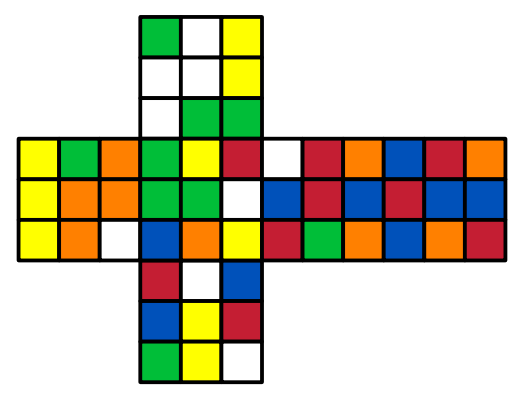
\includegraphics[width=8cm]{img/cubes/cub-barrejat.png}
    \caption{Cub barrejat per exemple de Memorització}
    \label{fig:exemple-memo}
    \end{figure}


